\documentclass[12pt,twocolumn]{article}
\usepackage[utf8x]{inputenc}
\usepackage[spanish, es-tabla]{babel}
\usepackage{graphicx}

\usepackage{amsmath}

\title{Proyecto Final}
\author{Juan B. Benavides y Juan P. Vanegas }
\date{\today}

\begin{document}
\maketitle

\section{\label{sec: Intro} Sistema Físico}
La entropía es uno de los conceptos físicos más difíciles de comprender. Para llegar a él se puede ver desde el punto de vista termodinámico, o desde un punto de vista más cercano a la teoría de la información. A partir de este segundo camino podemos definir la entropía como la cantidad de información que nos hace falta, en promedio, para saber la posición y velocidad de todas las moléculas (J.D. Muñoz). 

En este informe se estudiara la entropía de un sístema difusivo y se estudiara como se relaciona con el estado de equilibrio del sístema. Se comienza con una taza de café a la que se le echa una gota de crema en el centro. Por simplicidad se asumira que se tiene una taza bidimensional con una distribución inicial de crema como la mostrada en la figura \ref{fig:t0}. Las figuras \ref{fig:t1e4}, \ref{fig:t1e5} y \ref{fig:t1e6} muestran como evoluciona la difusión de la crema usando un algoritmo de Random Walk. Se asume que en las posiciones $x = \pm 100$, y $y= \pm 100$ hay paredes y por lo tanto la crema esta confinada a permanecer en dicho espacio.

\begin{figure*}\label{fig:t0}
    \centering
    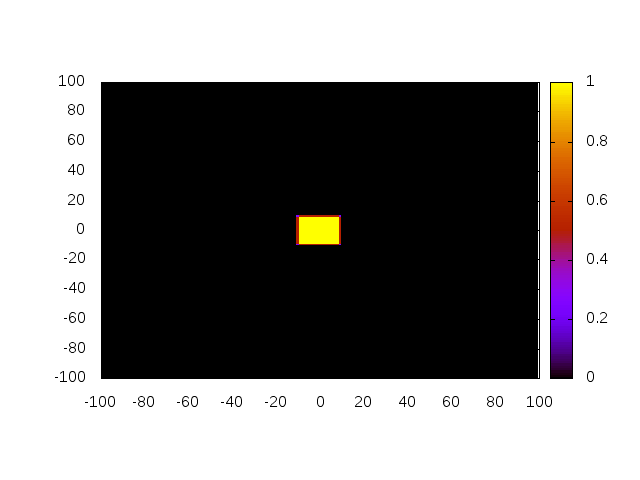
\includegraphics[width=0.75\textwidth]{figs/t_0.png}
    \caption{Configuración inicial usando algoritmo procedimental con 400 particulas de crema.}
\end{figure*}

\begin{figure*}\label{fig:t1e4}
    \centering
    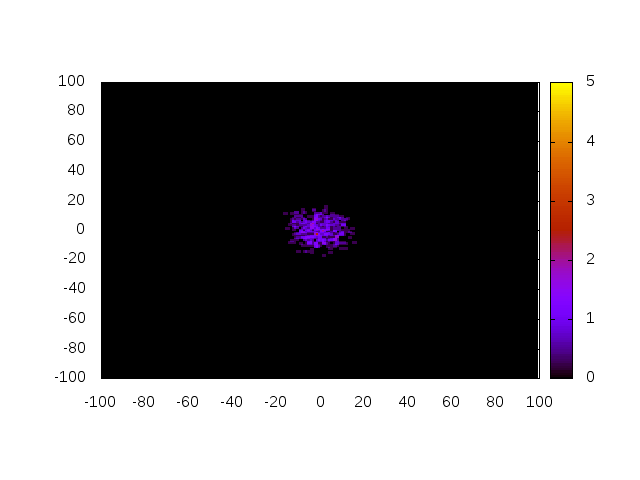
\includegraphics[width=0.75\textwidth]{figs/t_1e4.png}
    \caption{Difusión después de $10^4$ pasos de tiempo usando 
        algoritmo procedimental con 400 particulas de crema}
\end{figure*}

\begin{figure*}\label{fig:t1e5}
    \centering
    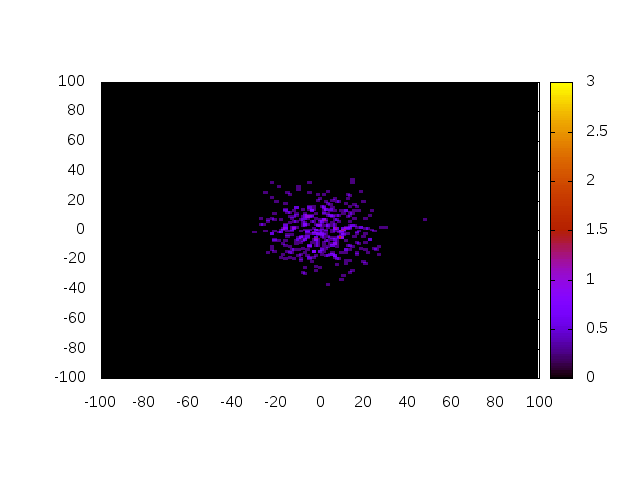
\includegraphics[width=0.75\textwidth]{figs/t_1e5.png}
    \caption{Difusión después de $10^5$ pasos de tiempo usando 
        algoritmo procedimental con 400 particulas de crema}
\end{figure*}

\begin{figure*}\label{fig:t1e6}
    \centering
    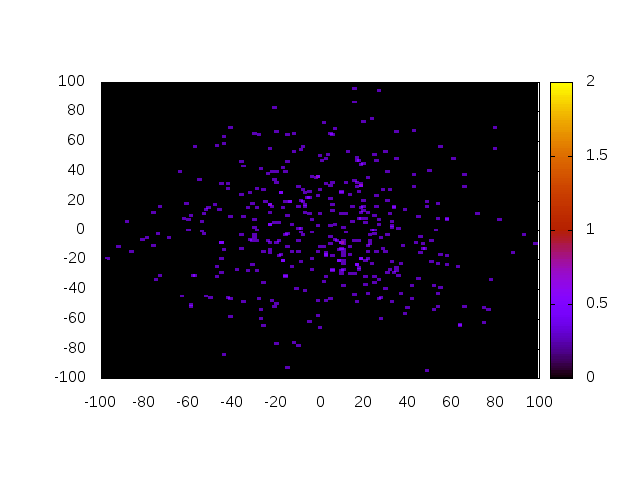
\includegraphics[width=0.75\textwidth]{figs/t_1e6.png}
    \caption{Difusión después de $10^6$ pasos de tiempo usando 
        algoritmo procedimental con 400 particulas de crema}
\end{figure*}

Estas imagenes muestran como se reproduce un proceso difusivo usando esta simulación, sin embargo, nos interesa ir más allá y estudiar en este sistema la segunda ley de la termodinámica y como esta se relaciona a la forma en que el sistema se acerca al equilibrio. Recordemos que la mecánica estadistica establece que la entropía de un sistema cerrado siempre aumenta o permanece constante y que permanece constante solo cuando el sístema se encuentra en equilibrio termodinámico.

Para medir la entropía se divide el espacio en celdas y se calcula la probabilidad $P$ de que haya una molécula en una celda dada contando el numero de moleculas en la celda y dividiendo entre el número total de moléculas. Luego, la entropía se calcula según la definición usual de la mecánica estadística como: 

\begin{equation} \label{eq: Entropy}
	S = - \sum _i P_i \log{P_i}
\end{equation}

En este caso, se suma sobre todas las moléculas y se mide la probabilidad de que cada molécula se encuentre en una celda dada. Si la probabilidad de que la molécula este en una celda es cero, esa celda no se tienen en cuenta para evitar el error en el logarítmo. 
\section{Algoritmos y \\ Validación}

Para modelar este fenómeno utilizamos dos paradigmas de programación diferentes: Procedimental 
y Orientado a Objetos, cada uno utilizando un algoritmo de propagación diferente. El 
algoritmo utilizado para el paradigma procedimental, descrito en la figura 
\ref{fig:algoritmo_Proc}, que consta en un arreglo de moléculas, donde cada elemento tiene 
la posición en x y y de una molécula. Para evolucionar el sistema se elige al azar una molécula, 
y se modifica su posición, de manera que se mueva una unidad en alguna dirección aleatoria. 
Este procedimiento de elegir una molécula y moverla se toma como un paso de tiempo.
\\
\begin{figure*}
    \centering
    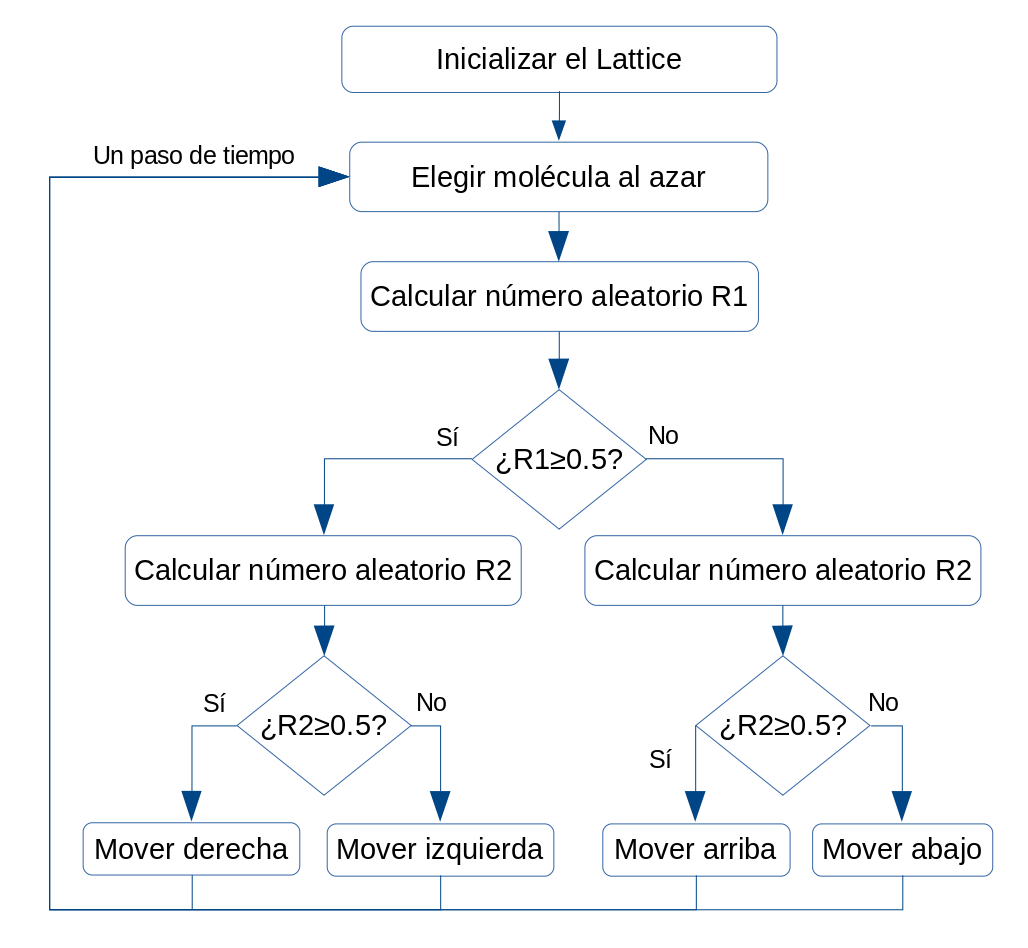
\includegraphics[width=0.75\textwidth]{figs/Algoritmo_Proc.png}
    \caption{Algoritmo 1.}
    \label{fig:algoritmo_Proc}
\end{figure*}

Por otro lado, para el paradigma orientado a objetos se implementó el algoritmo descrito 
en la figura \ref{fig:algoritmo_OOP}, que consiste en una matriz bidimesional de enteros no 
negativos, o Lattice, donde se representan las moléculas como el número de cada celda. Para 
mover las moléculas se recorre el Lattice celda por celda, y en caso de que se encuentre al 
menos una molécula en una celda se mueve a alguna casilla inmediatamente adyacente a la celda. 
Utilizando este algoritmo se toma un paso de tiempo está dado por un recorrido completo al 
Lattice, a diferencia del criterio empleado en el paradigma procedimental. 
\\

Dos factores a considerar en este algoritmo es que, primero, en dado caso que una molécula 
al desplazarse se ubique en la celda donde el algoritmo continúa buscando, esta se moverá 
dos veces. Este caso, aunque poco probable, conlleva a una ligera pérdida de información 
frente al algoritmo procedimental. 
\\

En segundo lugar, dado que un paso de tiempo del paradigma orientado a objetos implica 
mover aproximadamente todas las moléculas, cada paso de tiempo de este algoritmo es N veces 
más rápido que el algoritmo procedural, con N el número inicial de moléculas. Por lo tanto, 
cualquier cálculo que se realize en función del tiempo se verá directamente afectado, 
resultando en que el algoritmo orientado a objetos solo calcula una variable cada 400 
cálculos del algoritmo procedural. Este factor sí debe tenerse en cuenta, y solo puede 
ser despreciado en caso de que el tiempo computacional total que se deba utilizar para 
hallar resultados concluyentes sea mucho mayor a 400.
\\
\begin{figure*}
    \centering
    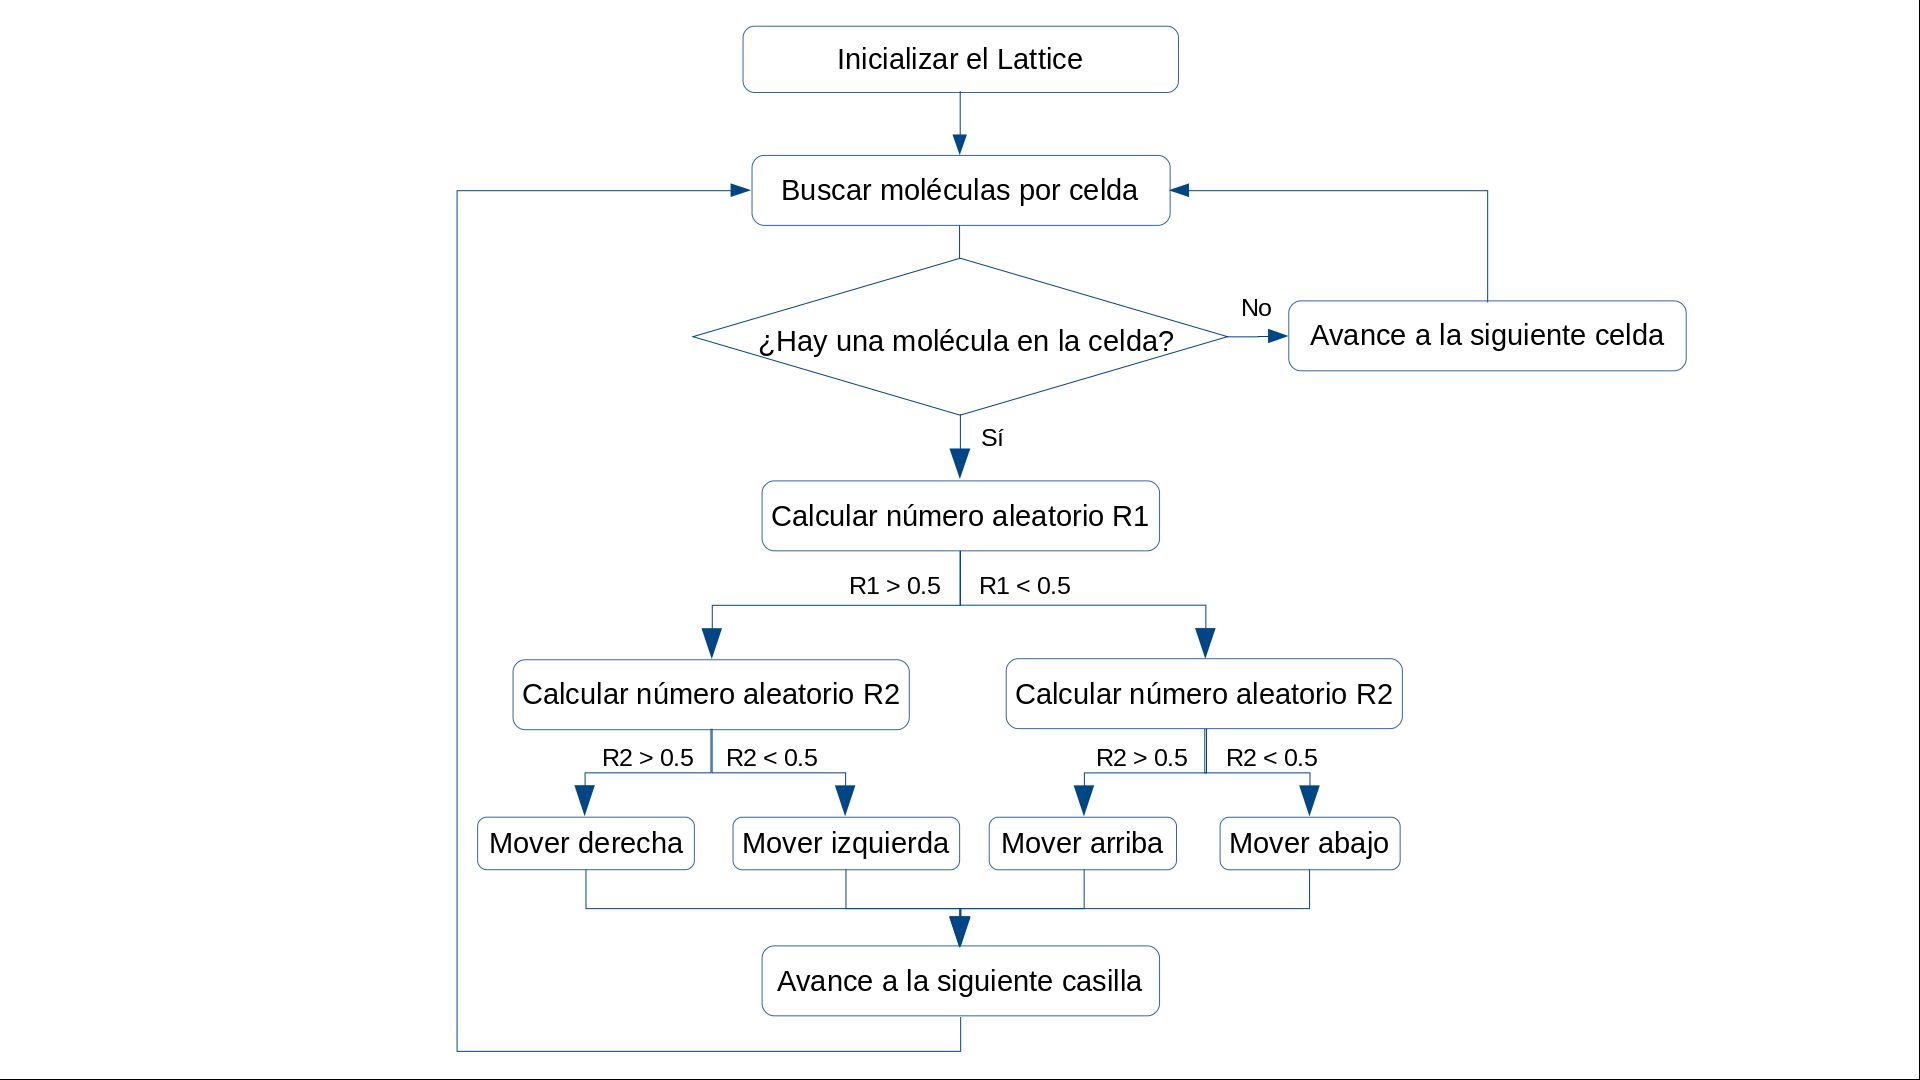
\includegraphics[width=0.75\textwidth]{figs/Algoritmo_OOP.png}
    \caption{Algoritmo 2.}
    \label{fig:algoritmo_OOP}
\end{figure*}

Para validar cada uno de estos métodos se calculó la entropía usando la ecuación \ref{eq: Entropy} en función del tiempo de cómputo, donde esperamos que inicialmente halla un crecimiento muy rápido de la entropía del sistema, que para este caso corresponde a la gota de crema difundiéndose por la taza. Luego esperamos que la entropía se estabilice y tenga un comportamiento asintótico alrededor de algún valor, que corresponde al momento en el que la crema se haya distribuido de manera más o menos uniforme alrededor de la taza y por lo tanto, el sistema llega al equilibrio.
\\
\begin{figure*}
    \centering
    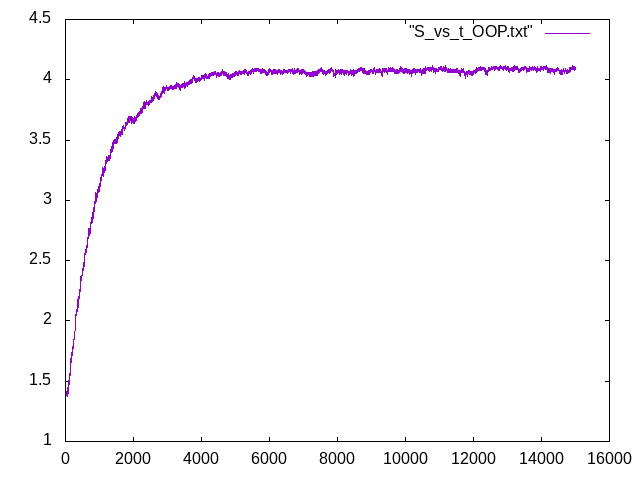
\includegraphics[width=0.75\textwidth]{figs/S_vs_t_OOP.png}
    \caption{Entropía en función del tiempo para paradigma orientado a objetos.}
    \label{fig:s_vs_t_OOP}
\end{figure*}
\begin{figure*}
    \centering
    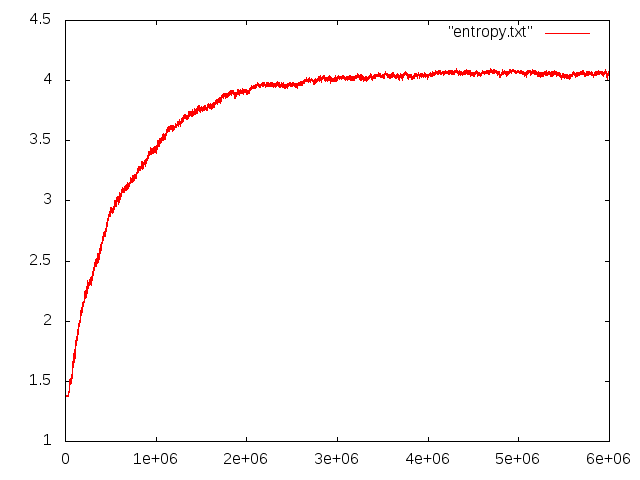
\includegraphics[width=0.75\textwidth]{figs/entropy.png}
    \caption{Entropía en función del tiempo para paradigma procedimental.}
    \label{fig:s_vs_t_Proc}
\end{figure*}

Vemos que en ambos paradigmas, y por lo tanto, algoritmos, el comportamiento de la entropía en función del tiempo es el esperado, por lo que ambos métodos quedan validados para modelar este sistema. Vemos también que el tiempo de computo total empleado para el paradigma orientado a objetos es mucho mayor a 400, con lo que también podemos despreciar la información perdida por utilizar este método. A partir de este punto se transformará el tiempo del paradigma orientado a objetos multiplicando el tiempo de cómputo por un factor de 400, lo que permite comparar directamente los resultados obtenidos en ambos paradigmas.

\section{Resultados y Análisis}

A continuación, ya teniendo los dos paradigmas validados para simular este sístema, se procede a estudiar distintos aspectos físicos.

En primer lugar, se estudia como depende el tiempo para el que se alcanza el equilibrio del tamaño de la taza. En la figura \ref{fig:S_vs_t_sizes} se ve como a medida que aumenta el tamaño del sístema, aumenta también el tiempo que le toma en llegar al equilibrio.

\begin{figure*}
    \centering
    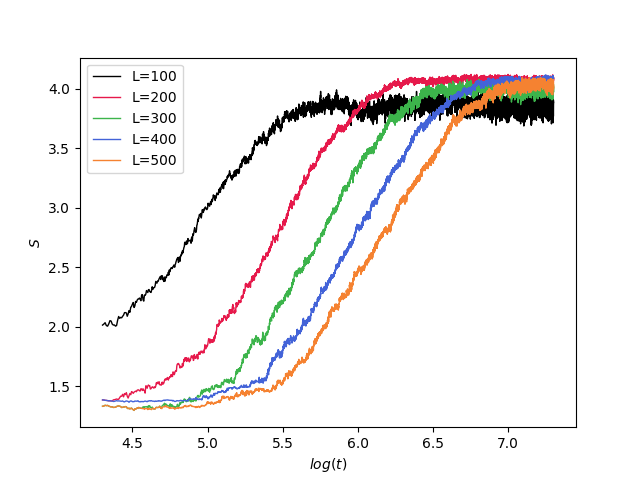
\includegraphics[width=0.75\textwidth]{figs/S_vs_t_sizes.png}
    \caption{Comparación de la Entropía en función del tiempo para diferentes tamaños de Lattice. Para mejorar la visualización, se gráfica el tiempo en escala logarítmica.}
    \label{fig:S_vs_t_sizes}
\end{figure*}

Por otro lado, el principio ergódico establece que en el equilibrio todos los estados son ocupados con igual probabilidad, lo que se da cuando la crema está distribuida uniformemente en todo el espacio. Esto concuerda con nuestro concepto intuitivo del equilibrio en este sístema. Para medir esto se estudia como varía el tamaño de la gota de crema en el tiempo. Esta medida se hace tomando la raiz del promedio de la distancia al orígen al cuadrado, es decir: 
\begin{equation*} \label{eq: root-mean}
	\sqrt{\frac{\sum_i r_i^2}{N}}
\end{equation*}
La figura \ref{fig:size_alone} muestra como va aumentando el tamaño de la gota de crema. 
\begin{figure*}
    \centering
    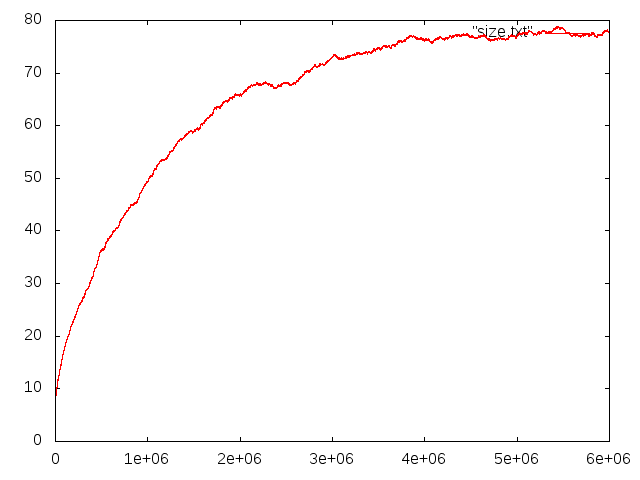
\includegraphics[width=0.75\textwidth]{figs/size_alone.png}
    \caption{En la imagen se puede ver el tamaño de la gota en función del tiempo.}
    \label{fig:size_alone}
\end{figure*}

Por otro lado, este resultado se puede usar para probar que la crema tiene un comportamiento difusivo en que el tamaño de la gota crece proporcional a $t^{1/2}$ hasta que se alcanza el equilibrio, momento en que dicho comportamiento cambia. Para ver esto se realiza una normalización del tamaño dividiendolo por una constante de forma que se pueda gráficar junto con la entropía para ver más claramente el resultado. luego se realiza un ajuste de los datos a una función de la forma $f(x)= at^{1/2} + b$. En la figura \ref{fig:size} se puede ver como el tamaño del sístema coincide perfectamente con el ajuste realizado hasta un poco antes de $t= 2\times 10^6$, tiempo en el que se puede ver que la entropía llega a su máximo y por tanto, se obtiene el equilibrio. En el ajuste obtenido se tiene $a=  0.002269$ y $b= 0.177329$.

\begin{figure*}
    \centering
    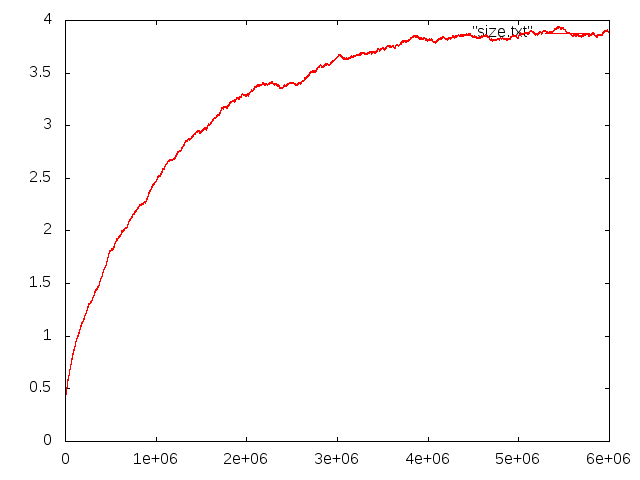
\includegraphics[width=0.75\textwidth]{figs/size.png}
    \caption{En la imagen se puede ver el tamaño de la gota (se normaliza dividiendolo entre 20 para que se pueda comparar con la entropía), la función $0.002269 \sqrt{t} + 0.177329$ y la entropía del sístema.}
    \label{fig:size}
\end{figure*}

Finalmente, consideremos lo que sucedería si la taza tiene un hueco en un lado y por lo tanto cuando las partículas llegan a dicho hueco, desaparecen. En este caso se debe observar como el número de partículas que hay en la taza disminuye como $\exp{(\frac{t}{\tau})}$. Esto se puede ver en la figura \ref{fig:hole} donde se gráfica el número de partículas contra el tiempo junto con un ajuste de los datos en el que se obtiene un parametro $\tau = 55433.6\mathrm{s}$.
\begin{figure*}
    \centering
    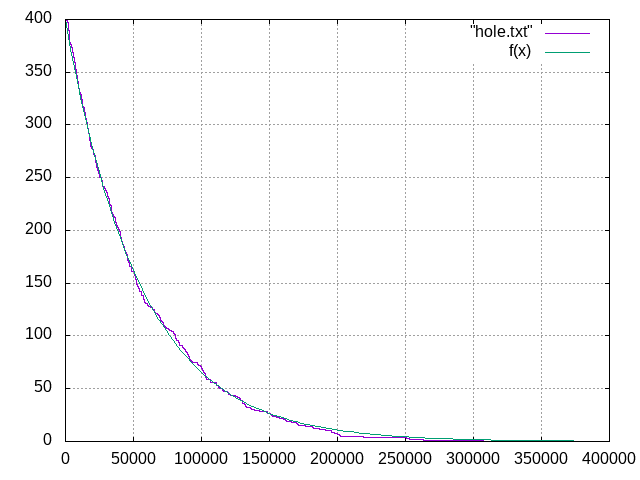
\includegraphics[width=0.75\textwidth]{figs/hole.png}
    \caption{Propagación de las moléculas con un agujero en la pared.}
    \label{fig:hole}
\end{figure*}



\section{Conclusiones}
\begin{itemize}
    \item 
\end{itemize}

\end{document}
